% ============================================================================
%  Reading the convergence rate off the decomposition structure
%  treewidth as the easy/hard axis for Z_L = sum_{|I|=L} omega(I)
%
%  Self-contained note (references in footnotes); no .bib needed.
%      pdflatex classification.tex   (twice, for cross-references)
%  Figures: code/exp5_classification.py, code/exp6_exponent.py.
% ============================================================================
\documentclass[11pt]{article}

\usepackage[a4paper, margin=1in]{geometry}
\usepackage{amsmath, amssymb, amsthm, mathtools, bm}
\usepackage{graphicx}
\usepackage{booktabs}
\usepackage{array}
\usepackage[dvipsnames]{xcolor}
\usepackage{enumitem}
\usepackage{tikz}
\usetikzlibrary{arrows.meta, decorations.pathreplacing}
\usepackage[colorlinks=true, linkcolor=NavyBlue!70!black,
            urlcolor=BrickRed!70!black]{hyperref}

\newcommand{\R}{\mathbb{R}}
\newcommand{\tr}{\operatorname{tr}}
\newcommand{\tw}{\operatorname{tw}}
\newcommand{\eqdef}{\coloneqq}
\newcommand{\one}{\mathbf 1}
\newcommand{\spec}{\rho}
\newcommand{\F}[1]{\smallskip\noindent\textbf{\textsf{#1.}}\hspace{0.4em}}

\theoremstyle{plain}
\newtheorem{lemma}{Lemma}
\newtheorem{corollary}[lemma]{Corollary}
\theoremstyle{definition}
\newtheorem{principle}[lemma]{Diagnostic}

\setlist{leftmargin=1.6em}

\title{\bf Reading the convergence rate off the decomposition structure\\[2pt]
       \large treewidth as the easy/hard axis for $Z_L=\sum_{|I|=L}\omega(I)$}
\date{\today}

\begin{document}
\maketitle
\vspace{-1.4em}

\begin{abstract}\noindent
Many ``rates'' are the growth rate $\lambda=\lim_L Z_L^{1/L}$ of a sum over
length-$L$ words, $Z_L=\sum_{|I|=L}\omega(I)$. This note makes one claim
precise: \emph{the decomposition structure of $Z_L$ -- the treewidth of the
graph that records which indices its weight couples -- tells you the
\textbf{nature and difficulty} of the rate before you compute a single digit.}
It does \textbf{not} tell you the numerical value; it tells you whether the rate
is an exactly-computable eigenvalue, whether it is likely algebraic or
transcendental, what kind of corrections to $\lambda^L$ to expect (geometric vs.\
a power law $L^\theta$), and what it costs to get it. The cleanest payoff is at
the hard end: when no finite transfer matrix exists, the same picture says how
far you can push $Z_L$ and how to \emph{verify a conjectured exponent} -- which is
exactly how the 2D self-avoiding-walk exponent $11/32$ is corroborated.
\end{abstract}

% ===========================================================================
\section{The question}
% ===========================================================================

Write $Z_L=\sum_{I\in\mathcal W_L}\omega(I)$ as a tensor contraction (an
\textsc{einsum}) and let $G_L$ be its \emph{dependency graph}: one vertex per
summation index, an edge between two indices whenever they appear together in a
factor of $\omega$.\footnote{This is the decomposition graph of the companion
$U$-statistics paper, here indexed by the growing word length $L$ rather than a
fixed kernel order.} The cost of evaluating one $Z_L$ by optimal index
elimination is $\Theta\!\bigl(q^{\,\tw(G_L)+1}\bigr)$ per site, where $q$ is the
alphabet size and $\tw$ is the treewidth.\footnote{S.~A.~Markov and Y.~Shi,
\emph{SIAM J.\ Comput.}\ (2008); the treewidth/contraction link is classical in
graphical models. Finding the optimal order is NP-hard (Arnborg--Corneil--%
Proskurowski, 1987), which is why solvers use heuristics.} The whole question is
how $\tw(G_L)$ behaves as $L\to\infty$.

\begin{center}
\fbox{\parbox{0.93\textwidth}{\centering
\emph{Bounded treewidth} $\Longleftrightarrow$ a \emph{finite transfer
matrix} carries the weight $\Longleftrightarrow$ the rate is an
\emph{eigenvalue}.\\[2pt]
\emph{Growing treewidth} $\Longleftrightarrow$ \emph{no} finite carrier
$\Longleftrightarrow$ the rate is only \emph{estimable}, and a power law may
appear.}}
\end{center}

The rest of the note (i)~proves the one fact that makes the dichotomy sharp,
(ii)~refines it into three levels, (iii)~turns it into a decision procedure you
can run on the asymptotics, and (iv)~shows the payoff: verifying conjectured
orders.

% ===========================================================================
\section{The one fact: a finite carrier forbids a power law}
% ===========================================================================

Suppose the family is \emph{transfer-decomposable}: there is a fixed nonnegative
matrix $T$ and boundary vectors $u,v$ with
\begin{equation}
\label{eq:transfer}
   Z_L=\langle u,\,T^{L}\,v\rangle\qquad\text{for all }L.
\end{equation}
This is exactly what bounded treewidth buys (for a linearly ordered family): the
state is the set of ``live'' indices at a cut, of which there are at most
$q^{\,\tw}$.

\begin{lemma}[finite carrier $\Rightarrow$ pure geometric corrections]
\label{lem:main}
Let \eqref{eq:transfer} hold with $T$ primitive, simple top eigenvalue
$\lambda_1=\spec(T)$, second modulus $|\lambda_2|<\lambda_1$, and $u,v$ not
orthogonal to the Perron eigenvectors. With $\delta\eqdef|\lambda_2|/\lambda_1\in[0,1)$,
\[
   \boxed{\;Z_L=c\,\lambda_1^{L}\bigl(1+O(\delta^{L})\bigr),\qquad
   \frac{Z_L}{\lambda_1^{L}}\xrightarrow[L\to\infty]{}c>0.\;}
\]
In particular a finite primitive carrier \textbf{cannot} produce a nontrivial
power-law factor $L^{\theta}$.
\end{lemma}

\begin{proof}
Perron--Frobenius makes $\lambda_1$ simple with positive eigenvectors $w_R,w_L$
($\langle w_L,w_R\rangle=1$); the spectral decomposition is
$T^{L}=\lambda_1^{L}\Pi+R^{L}$ with $\Pi=w_Rw_L^{\!\top}$ rank one and
$\spec(R)=|\lambda_2|$. Then
$Z_L=\lambda_1^{L}\langle u,w_R\rangle\langle w_L,v\rangle+\langle u,R^{L}v\rangle$,
and $\|R^{L}\|=O(|\lambda_2|^{L})$ gives the claim with
$c=\langle u,w_R\rangle\langle w_L,v\rangle>0$.
\end{proof}

The contrapositive is the useful half, because it is something you can
\emph{observe}:

\begin{corollary}[a power law certifies entanglement]
\label{cor:certificate}
If $Z_L/\lambda^{L}$ does not tend to a positive constant -- e.g.\ it drifts like
$L^{\theta}$ with $\theta\neq0$, or the ratio $Z_{L+1}/Z_L$ approaches its limit
only \emph{algebraically} ($\sim 1/L$) instead of \emph{geometrically} -- then no
finite primitive transfer matrix represents the family. The carrier is infinite
and its spectrum has no gap (continuous spectrum, or criticality
$\delta\to1$).\footnote{If $\lambda_2$ sits in a Jordan block the error gains a
factor $L^{b-1}$, but the \emph{leading} term keeps $c>0$ because primitivity
makes $\lambda_1$ simple; so a persistent $L^\theta$ multiplying $\lambda^L$ is
still impossible.}
\end{corollary}

Figure~\ref{fig:diagnostic} shows both sides on elementary, exactly known
sequences: the golden-mean count $Z_L=F_{L+2}$ (a \emph{local} constraint -- no
two adjacent $1$s -- hence a $2$-state carrier) against the central binomial
$Z_L=\binom{2L}{L}$ (a \emph{global} constraint -- equal numbers of $\pm1$ --
which forces the carrier to track an unbounded height, so there is none finite).
The first has $Z_L/\varphi^L\to\varphi^2/\sqrt5$ and a geometric ratio; the second
has $Z_L/4^L\sim(\pi L)^{-1/2}$ and a $1/L$ ratio. Same template, opposite
classes, and the class is legible in the picture.

\begin{figure}[h]
\centering
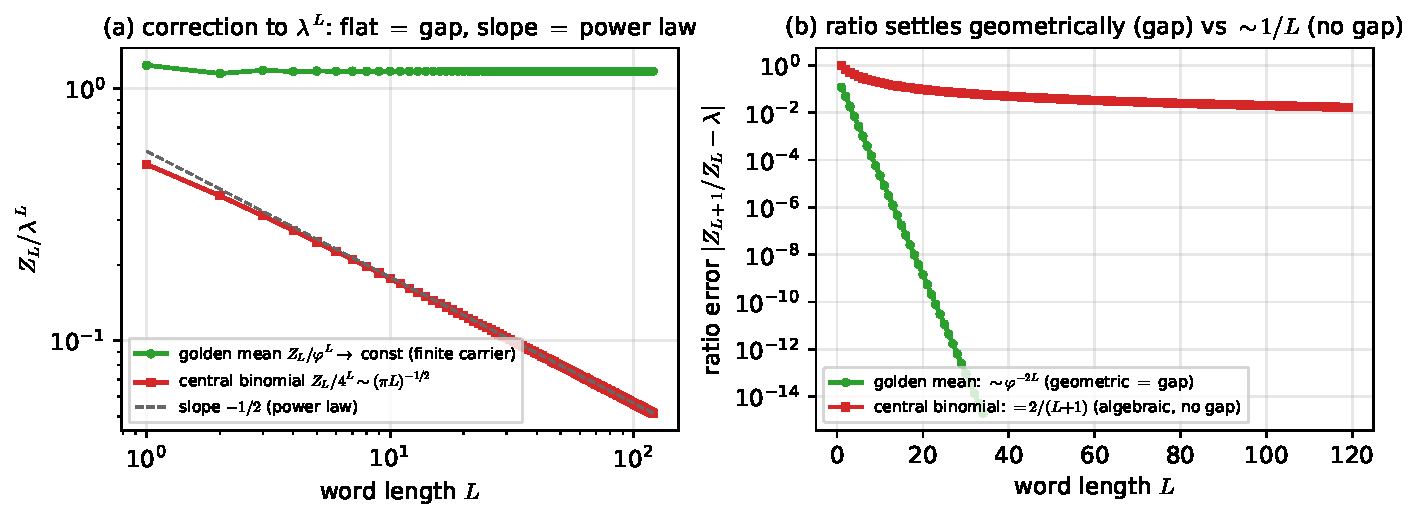
\includegraphics[width=\textwidth]{figures/classification.pdf}
\caption{The structural diagnostic (Corollary~\ref{cor:certificate}).
(a)~$Z_L/\lambda^L$ is \emph{flat} for a finite carrier (golden mean) and a
\emph{power law} of slope $-\tfrac12$ for the carrier-less central binomial.
(b)~the naive ratio $Z_{L+1}/Z_L$ settles \emph{geometrically} when there is a
gap and only as $\sim1/L$ when there is not. Local constraint vs.\ global
constraint $=$ bounded vs.\ growing carrier $=$ gap vs.\ no gap.}
\label{fig:diagnostic}
\end{figure}

% ===========================================================================
\section{The axis, in three levels}
% ===========================================================================

Treewidth is the first-order classifier; the sharp invariant underneath it is
\emph{``does a transfer operator with a spectral gap exist''}. Three levels:

\begin{figure}[h]
\centering
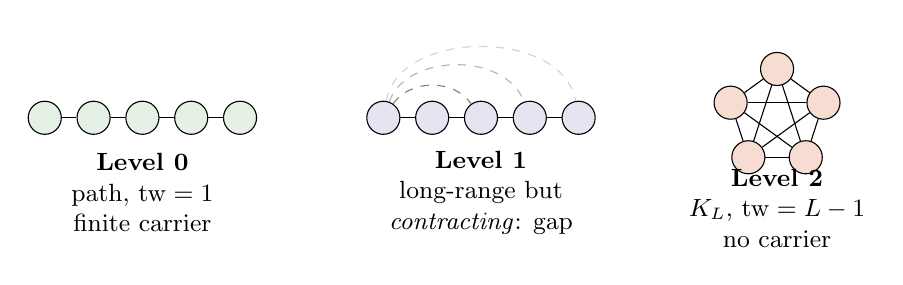
\begin{tikzpicture}[node distance=7mm, every node/.style={font=\small}]
\tikzset{v/.style={circle, draw, fill=ForestGreen!12, minimum size=4.2mm, inner sep=0}}
% --- Level 0: path ---
\begin{scope}[xshift=0cm]
  \foreach \i in {0,...,4} \node[v] (a\i) at (\i*0.62,0) {};
  \foreach \i [evaluate=\i as \j using int(\i+1)] in {0,...,3} \draw (a\i)--(a\j);
  \node[align=center] at (1.24,-0.95) {\textbf{Level 0}\\path, $\tw=1$\\finite carrier};
\end{scope}
% --- Level 1: path with decaying long-range (contracting) ---
\begin{scope}[xshift=4.3cm]
  \foreach \i in {0,...,4} \node[v,fill=NavyBlue!10] (b\i) at (\i*0.62,0) {};
  \foreach \i [evaluate=\i as \j using int(\i+1)] in {0,...,3} \draw (b\i)--(b\j);
  \draw[dashed,gray] (b0) to[bend left=55] (b2);
  \draw[dashed,gray!60] (b0) to[bend left=70] (b3);
  \draw[dashed,gray!35] (b0) to[bend left=80] (b4);
  \node[align=center] at (1.24,-0.95) {\textbf{Level 1}\\long-range but\\\emph{contracting}: gap};
\end{scope}
% --- Level 2: complete graph ---
\begin{scope}[xshift=9.3cm]
  \foreach \i in {0,...,4} \node[v,fill=BrickRed!12] (c\i) at ({90+\i*72}:0.62) {};
  \foreach \i in {0,...,4} \foreach \j in {0,...,4} {\ifnum\i<\j \draw (c\i)--(c\j);\fi}
  \node[align=center] at (0,-1.15) {\textbf{Level 2}\\$K_L$, $\tw=L-1$\\no carrier};
\end{scope}
\end{tikzpicture}
\caption{The dependency graph $G_L$ across the three levels: local coupling
(path), long-range-but-contracting coupling, and global coupling (complete
graph). Treewidth grows left to right.}
\label{fig:graphs}
\end{figure}

\F{Level 0 -- finite carrier} Bounded treewidth, finite alphabet, weight that
couples only nearby indices. The carrier $\Sigma$ is a \emph{finite} set,
$|\Sigma|\le q^{\,\tw}$, and \eqref{eq:transfer} holds with a genuine matrix.
\begin{itemize}[itemsep=1pt]
\item rate $=\spec(T)$, computed once and exactly; \textbf{algebraic} if the
weights are (a root of $\det(\lambda I-T)$);
\item $Z_L=\sum_i c_i\lambda_i^L$: corrections are \textbf{geometric}, no power
law (Lemma~\ref{lem:main});
\item cost of $Z_L$: $O(L\,q^{\,\tw+1})$, \emph{linear} in $L$; the
``divide-out-and-check-$\to1$'' heuristic is a \emph{theorem}.
\end{itemize}
Examples: subshift entropy, the golden-mean shift, 1D Ising/Potts free energy,
and -- at each fixed width -- a 2D model on a strip.

\F{Level 1 -- compact carrier with a gap} The naive treewidth looks unbounded
(each weight depends on the whole word through a composition), but the dynamics
is \emph{contracting} (hyperbolic / bounded distortion), which collapses the
weight onto a transfer \emph{operator} on a function space. That operator is
infinite-dimensional but trace-class with a \emph{spectral gap}.
\begin{itemize}[itemsep=1pt]
\item rate is a ``nice'' eigenvalue, typically \textbf{transcendental}, but
computable to arbitrary precision: finite truncations (Chebyshev collocation,
Fredholm/spectral determinants) converge \textbf{super-exponentially} for
real-analytic systems;
\item corrections still essentially geometric (the gap);
\item this is the regime of \emph{Bowen's formula} and Ruelle's thermodynamic
formalism.\footnote{R.~Bowen (1979); D.~Ruelle, \emph{Thermodynamic Formalism};
V.~Baladi, \emph{Positive Transfer Operators} (2000).}
\end{itemize}
Examples: $\dim_H E_2=0.5312805062772\ldots$ (the continued-fraction
set),\footnote{O.~Jenkinson and M.~Pollicott, \emph{Adv.\ Math.}\ (2001) and the
``hundred digits'' computation (2018).} the Gauss--Kuzmin--Wirsing constant
($\approx0.3036$, literally a spectral gap), conformal Hausdorff dimensions, and
top Lyapunov exponents \emph{under a domination/cone condition} -- the condition
is precisely what restores the gap.

\F{Level 2 -- no gap / growing essential treewidth} No transfer operator with a
gap exists. Either the treewidth grows ($\tw(G_L)=\Theta(L)$ for global coupling
such as $K_L$, or $\Theta(W)$ on a width-$W$ strip), or the spectrum is
continuous / the system is critical.
\begin{itemize}[itemsep=1pt]
\item the rate is only \textbf{estimable}, by brute force over $q^{\Theta(L)}$
words (or $q^{\Theta(W)}$ strip states) followed by series analysis;
\item \textbf{power-law} (or stranger) corrections appear -- the fingerprint of
Corollary~\ref{cor:certificate};
\item the value can be transcendental, or worse: for the joint spectral radius,
deciding $\spec\le1$ is \emph{undecidable} and the finiteness conjecture is
\emph{false}.\footnote{V.~Blondel and J.~Tsitsiklis (2000); T.~Bousch and
J.~Mairesse (2002).}
\end{itemize}
Examples: self-avoiding walks, lattice animals/polyominoes, pattern-avoiding
permutations, the affinity dimension of self-affine sets, the joint spectral
radius.

% ===========================================================================
\section{So: can you read the rate off the structure?}
% ===========================================================================

\emph{Its value, no. Its nature, cost, and the right way to attack it, yes.}
Concretely, the structure fixes four things in advance:

\begin{center}
\renewcommand{\arraystretch}{1.25}
\small
\begin{tabular}{@{}lccc@{}}
\toprule
 & \textbf{Level 0} & \textbf{Level 1} & \textbf{Level 2}\\
\midrule
$\tw(G_L)$ as $L\to\infty$ & bounded & bounded\,$^\ast$ & growing\\
rate is\ldots & algebraic eigenvalue & transcendental, gapped & estimate only\\
correction to $\lambda^L$ & geometric & geometric & power law / stranger\\
cost of $Z_L$ & $O(L)$ & $O(L)$, precision cheap & $q^{\Theta(L)}$ / $q^{\Theta(W)}$\\
``divide-out'' heuristic & theorem & theorem & heuristic (but standard)\\
\bottomrule
\end{tabular}
\end{center}
{\footnotesize $^\ast$ the \emph{combinatorial} treewidth looks unbounded;
the \emph{effective} dimension is finite because of contraction.}

\begin{principle}[a decision procedure]
\label{diag:procedure}
Given $Z_L$:
\textbf{(1)} draw $G_L$ and gauge $\sup_L\tw(G_L)$ -- local coupling is bounded,
global coupling ($K_L$) grows;
\textbf{(2)} if the weight is a smooth contraction of an a-priori long word
(derivatives, products of matrices through a \emph{linear} functional, conformal
maps), suspect Level 1, not Level 2;
\textbf{(3)} \emph{confirm from the data}: compute $Z_{L+1}/Z_L$. If it settles
\emph{geometrically} you have a gap (Level 0/1) and the rate is an eigenvalue you
should compute directly; if it settles only as $\sim1/L$ (a power law in $Z_L$)
you are in Level 2 and must enumerate and fit.
\end{principle}

Step (3) is the bridge between the two halves of Figure~\ref{fig:diagnostic}:
the \emph{shape} of the approach to $\lambda$ is a measurement of the structural
class.

% ===========================================================================
\section{The payoff: verifying a conjectured order}
% ===========================================================================

The most valuable use is exactly where the rate is \emph{not} known: Level 2,
where one has a \emph{conjectured} asymptotic
\begin{equation}
\label{eq:ansatz}
   Z_L\;\sim\;A\,\lambda^{L}\,L^{\theta}
\end{equation}
and wants to test it. (In Level 0/1 there is nothing to fit -- the rate is an
eigenvalue and $\theta=0$ by Lemma~\ref{lem:main}.) The standard tool is the
\emph{ratio method}: from $r_L=Z_{L+1}/Z_L=\lambda\bigl(1+\theta/L+O(L^{-2})\bigr)$,
\begin{equation}
\label{eq:ratio}
   \theta_L\eqdef L\Bigl(\frac{r_L}{\lambda}-1\Bigr)\xrightarrow[L\to\infty]{}\theta,
   \qquad
   \theta_L^{(1)}\eqdef L\,\theta_L-(L-1)\theta_{L-1}\ \ (\text{one Richardson step})
\end{equation}
converges to $\theta$ faster ($O(L^{-2})$). Figure~\ref{fig:exponent} validates
this on two sequences whose exponent is \emph{known}: the central binomial
($\theta=-\tfrac12$) and the Catalan numbers ($\theta=-\tfrac32$); the
accelerated estimate pins each to several digits from $\sim100$ terms.

\begin{figure}[h]
\centering
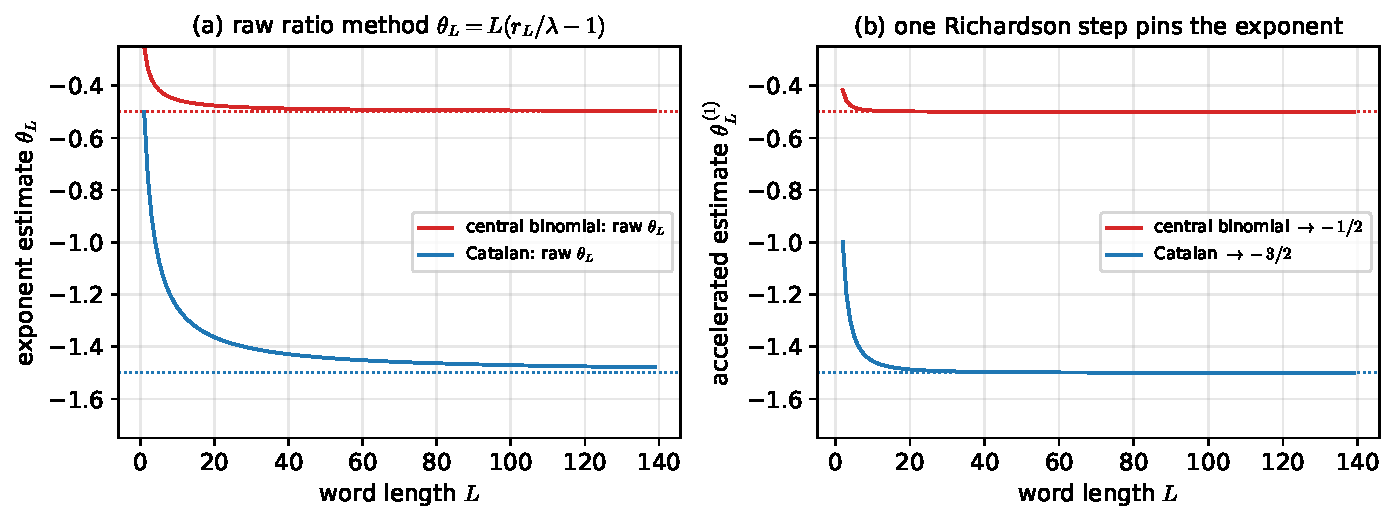
\includegraphics[width=\textwidth]{figures/exponent_fit.pdf}
\caption{Extracting the order $\theta$ from $Z_L$ alone, on cases with a known
answer. (a)~the raw ratio estimate $\theta_L$; (b)~one Richardson step pins
$\theta=-\tfrac12$ (central binomial) and $\theta=-\tfrac32$ (Catalan). The same
procedure, run on enumerated counts where $\lambda,\theta$ are unknown, is how
conjectured exponents are corroborated.}
\label{fig:exponent}
\end{figure}

\noindent The genuinely open / numerically settled problems where this is
\emph{the} method:

\begin{itemize}[itemsep=2.5pt]
\item \textbf{Self-avoiding walks (2D), the exponent $\tfrac{11}{32}$.}
$c_L\sim A\,\mu^{L}L^{\gamma-1}$ with $\gamma=\tfrac{43}{32}$, so
$\theta=\gamma-1=\tfrac{11}{32}=0.34375$, predicted by the Coulomb gas and
$\mathrm{SLE}_{8/3}$.\footnote{B.~Nienhuis (1982); Lawler--Schramm--Werner
(2004). The honeycomb connective constant $\mu=\sqrt{2+\sqrt2}$ is a theorem
(Duminil-Copin--Smirnov, 2012); the square-lattice $\mu$ and the exponent are
not.} The counts $c_L$ are produced by a \emph{finite-lattice transfer matrix}
on a strip of width $W$ -- a Level-2 family whose treewidth is the strip width --
to $L\approx80$, and \eqref{eq:ratio} (with differential approximants)
corroborates $11/32$.\footnote{I.~Jensen (2004); A.~J.~Guttmann (ed.),
\emph{Polygons, Polyominoes and Polycubes} (2009).} Here the treewidth
\emph{is} the budget: the reachable $L$, hence the precision on $\theta$, is set
by the affordable strip width $q^{\Theta(W)}$.
\item \textbf{$1324$-avoiding permutations -- a \emph{stretched} exponential.}
The Stanley--Wilf limit is $\mu\approx11.60$, but $\sim50$ computed terms reveal
the exotic form $B\,\mu^{L}\mu_1^{\sqrt L}L^{g}$ -- a correction $\mu_1^{\sqrt L}$
no finite matrix could ever produce, a vivid instance of
Corollary~\ref{cor:certificate}.\footnote{A.~Conway, A.~Guttmann and
P.~Zinn-Justin (2018).}
\item \textbf{Lattice animals / polyominoes.} Growth constant
$\lambda\approx4.0625697$ with conjectured exponent $\theta=-1$ in 2D, from
enumeration to large size and series analysis.\footnote{I.~Jensen (2003).}
\item \textbf{Joint spectral radius and affinity dimension.} Conjectured
extremal values and dimension formulas, tested on finite products $T_I$; the
honest boundary, where ``verify the order'' can be provably impossible
(undecidability).
\end{itemize}

The framework's contribution to this column is threefold: it \emph{certifies}
that these problems have no finite carrier (so an exponent $\theta\neq0$ is
expected, not an artifact); it gives the \emph{complexity scale} -- the treewidth
of the enumeration graph -- that fixes how far $L$, and hence how sharp $\theta$,
can go; and the contraction-order optimizers that solve the scheduling half
(\texttt{opt\_einsum}, \texttt{cotengra}) are literally the tools that maximize
the reachable $L$.\footnote{D.~G.~A.~Smith and J.~Gray (2018); J.~Gray and
S.~Kourtis (2021).}

% ===========================================================================
\section{What the structure does \emph{not} tell you}
% ===========================================================================

To keep the claim honest:
\begin{itemize}[itemsep=2pt]
\item \textbf{Not the value.} Two Level-0 families have different
eigenvalues; treewidth fixes the \emph{class}, never the number.
\item \textbf{Combinatorial treewidth can be too pessimistic.} Level 1 is exactly
the case where the naive graph looks entangled but a \emph{dynamical} gap
(contraction, domination) makes it easy. Detecting that gap is an analytic fact,
not a graph computation -- it is the rigorous content behind a practitioner's
hope that a weight ``approximately factorises''.
\item \textbf{The fit is heuristic.} In Level 2 the ratio/series method is an
extrapolation, not a proof; it can mislead (e.g.\ a $\sqrt L$ stretch hiding as a
slowly drifting $\theta$), which is why the $1324$ story took many terms.
\item \textbf{Optimal elimination is NP-hard}, and the worst Level-2 problems are
genuinely intractable (undecidable joint spectral radius).
\end{itemize}

\noindent In one line: \emph{treewidth is the axis that says whether a
convergence rate collapses to an eigenvalue or must be hunted by enumeration --
and in the latter case, how big the hunt is and how to read the conjectured
order off the catch.}

\bigskip
\noindent\textit{Reproduce:} \texttt{python3 code/run\_all.py}; Figures
\ref{fig:diagnostic}--\ref{fig:exponent} are \texttt{exp5\_classification.py} and
\texttt{exp6\_exponent.py}.

\end{document}
